\documentclass[11pt, a4paper]{article}

\usepackage[T1]{fontenc}
\usepackage[utf8]{inputenc}
\usepackage{lmodern}
\usepackage[a4paper, top=30mm, bottom=30mm, left=28mm, right=28mm]{geometry}
\usepackage{microtype}
\usepackage{parskip}
\usepackage{titlesec}
\usepackage{titling}
\usepackage[table]{xcolor}
\usepackage{tikz}
\usepackage{pgfplots}
\usepackage{hyperref}
\usepackage{enumitem}
\usepackage{booktabs}
\usepackage{array}
\usepackage{tabularx}
\usepackage{fancyhdr}
\usepackage{graphicx}
\usepackage{mdframed}
\usepackage{amsmath}

\usetikzlibrary{
  arrows.meta,
  positioning,
  shapes.geometric,
  shapes.misc,
  fit,
  backgrounds,
  decorations.pathreplacing,
  calc,
  shadows
}

\pgfplotsset{compat=1.18}

% ── Colour palette — MeshWhisper brand (teal) ────────────────────────────────
% Anchored to the brand 900 / 500 / 100 stops used in the site & SDK.
\definecolor{mwblue}{HTML}{014451}    % brand 900 — deep teal (title pages, headings)
\definecolor{mwaccent}{HTML}{0694A2}  % brand 500 — primary accent (links, accents)
\definecolor{mwbright}{HTML}{16BDCA}  % brand 400 — bright highlight
\definecolor{mwlight}{HTML}{D5F5F6}   % brand 100 — pale background
\definecolor{mwpale}{HTML}{EDFAFA}    % brand 50  — palest background
\definecolor{mwgray}{HTML}{6B7280}
\definecolor{mwrule}{HTML}{D1D5DB}
\definecolor{mwgreen}{HTML}{0E7C5B}
\definecolor{mwred}{HTML}{C0392B}
\definecolor{mworange}{HTML}{E67E22}
\definecolor{mwpurple}{HTML}{6B4FA0}
\definecolor{mwyellow}{HTML}{F5A623}
\definecolor{nodebg}{HTML}{EDFAFA}    % brand-tinted node background
\definecolor{devicebg}{HTML}{F0FFF4}

% ── Typography ────────────────────────────────────────────────────────────────
\titleformat{\section}{\large\bfseries\color{mwblue}}{}{0em}{}[\vspace{-4pt}\color{mwrule}\rule{\linewidth}{0.6pt}\vspace{4pt}]
\titleformat{\subsection}{\normalsize\bfseries\color{mwblue}}{}{0em}{}
\titlespacing{\section}{0pt}{22pt}{8pt}
\titlespacing{\subsection}{0pt}{14pt}{4pt}

\setlength{\parindent}{0pt}
\setlength{\parskip}{7pt}

% ── Hyperref ──────────────────────────────────────────────────────────────────
\hypersetup{
  colorlinks=true,
  linkcolor=mwaccent,
  urlcolor=mwaccent,
  pdftitle={MeshWhisper: Messaging as Ambient Infrastructure},
  pdfauthor={MeshWhisper}
}

% ── Header / footer ───────────────────────────────────────────────────────────
\pagestyle{fancy}
\fancyhf{}
\renewcommand{\headrulewidth}{0pt}
\fancyfoot[C]{\small\color{mwgray}\thepage}
\fancyfoot[R]{\small\color{mwgray}MeshWhisper}

% ── Pull-quote box ────────────────────────────────────────────────────────────
\newmdenv[
  topline=false, bottomline=false, rightline=false,
  linewidth=3pt, linecolor=mwaccent,
  backgroundcolor=mwlight,
  innerleftmargin=14pt, innerrightmargin=14pt,
  innertopmargin=10pt, innerbottommargin=10pt,
  skipabove=12pt, skipbelow=12pt
]{pullquote}

% ─────────────────────────────────────────────────────────────────────────────
\begin{document}

% ── Title page ────────────────────────────────────────────────────────────────
\begin{titlepage}
  \pagecolor{mwblue}
  \color{white}
  \centering
  \vspace*{32mm}
  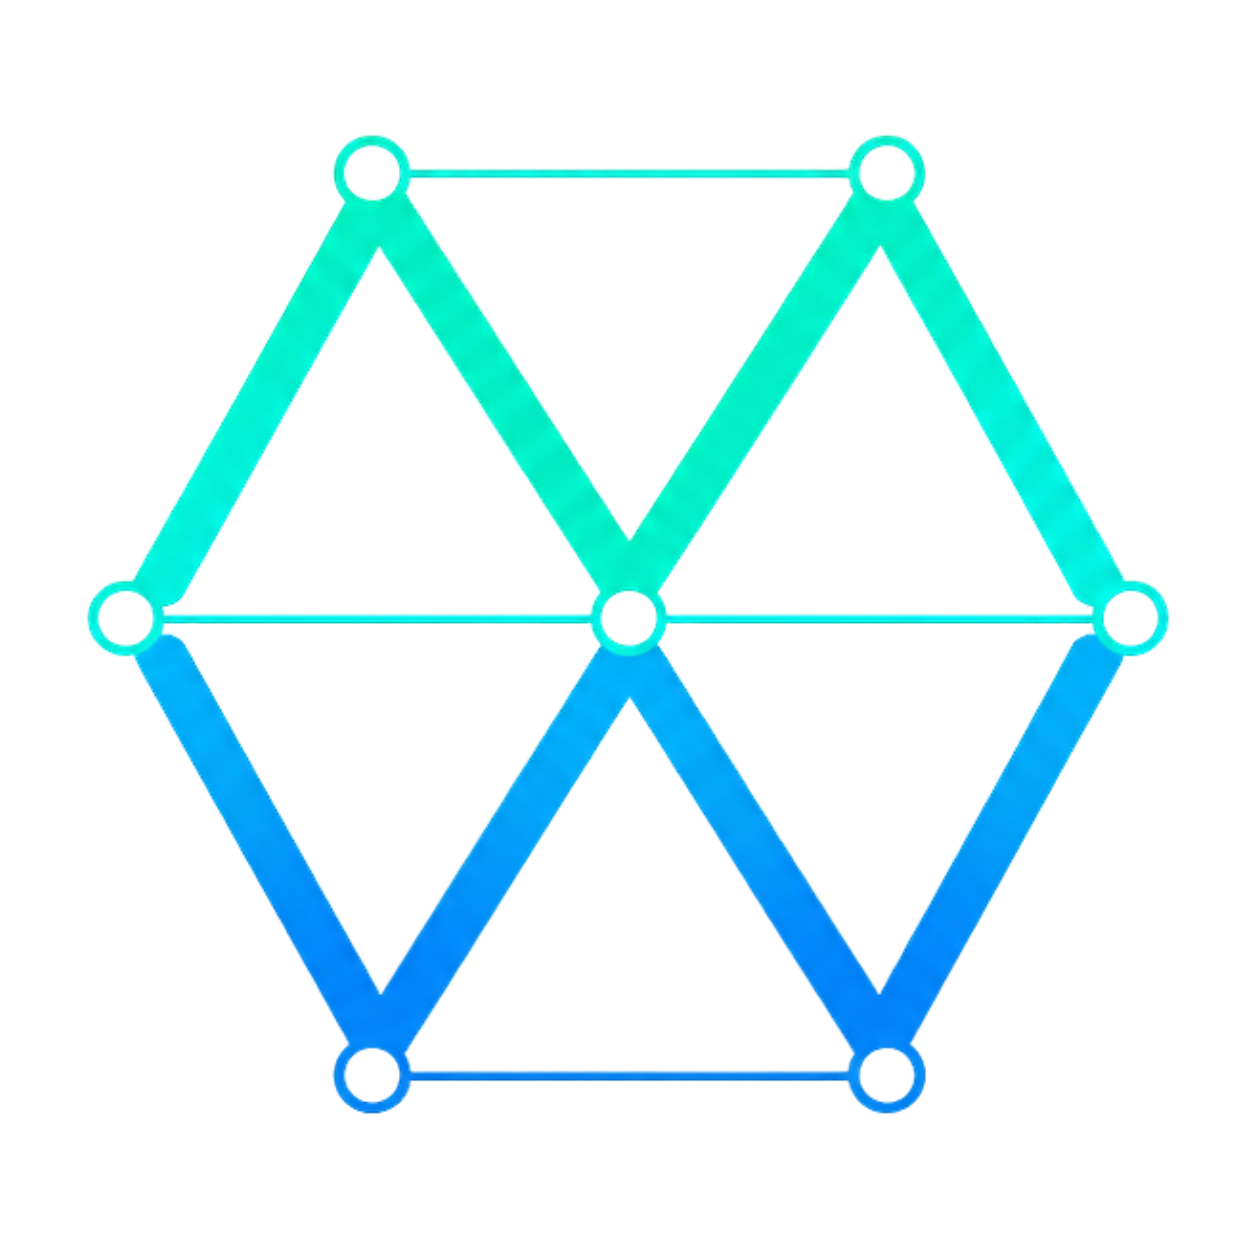
\includegraphics[width=46mm]{mw-logo-mark.png}\par
  \vspace{14mm}
  {\fontsize{30}{36}\selectfont\bfseries MeshWhisper\par}
  \vspace{6pt}
  {\fontsize{18}{24}\selectfont\color{mwbright} Messaging as Ambient Infrastructure\par}
  \vspace{20pt}
  {\color{mwbright}\rule{60mm}{1pt}}\par
  \vspace{20pt}
  {\color{white!85!mwblue}\normalsize April 2026\par}
  \vfill
  {\small\color{white!65!mwblue}
    Live: \texttt{relay.meshwhisper.org}\\
    Reference app: Prudence (\texttt{prudence.meshwhisper.org})\\
    \texttt{anton@gestureloop.com}\par
  }
\end{titlepage}

\pagecolor{white}
\color{black}
\setcounter{page}{1}

% ─────────────────────────────────────────────────────────────────────────────
\section{The Problem with Messaging Infrastructure}

Every application eventually needs messaging. A fitness app wants to connect athletes with coaches. A marketplace needs buyers to contact sellers. A coaching platform needs its members to coordinate. A community app needs its users to talk.

The developer faces the same choice every time.

\textbf{Build it yourself.} WebSocket servers are painful to build and expensive to scale. Real-time delivery, offline queuing, push notifications, media handling — each piece is a project on its own. Most small teams make a rational decision: skip messaging entirely, or redirect users to WhatsApp. The feature that would improve the product most is the one that never gets built.

\textbf{Pay for a managed service.} Sendbird starts at \$349/month. PubNub charges from \$98/month per thousand monthly active users. Stream Chat begins at \$119/month. These costs scale aggressively. An indie developer with fifty thousand users is looking at a four-figure monthly bill for infrastructure they didn't want to build in the first place. For most apps, the economics never work.

\textbf{Use Firebase or a general-purpose platform.} Free at small scale, but every message passes through Google's infrastructure in readable form. Legal liability. GDPR complexity. Vendor lock-in. And eventually, at the scale that matters, a pricing cliff.

This trilemma has a structural cause. Traditional messaging infrastructure is expensive because it has to be. A centralised server receives every message, processes it, stores it, and delivers it. That server reads every message in order to route it. Scale requires more servers. More servers cost money. The bill lands on the developer.

The assumption embedded in this model — that a central server must understand a message to route it — is the assumption MeshWhisper breaks.

% ─────────────────────────────────────────────────────────────────────────────
\section{The Core Insight}

A relay does not need to read a message to forward it.

If messages are encrypted before they leave the sending device, a relay is just a pipe. It receives an opaque blob, identifies the intended recipient by a hash, and forwards the blob. It cannot read the content. It does not need to. The message arrives at the recipient's device and is decrypted there, locally, with a key the relay never held.

This is not a novel observation in isolation. Signal uses end-to-end encryption. So does WhatsApp. The difference is that Signal and WhatsApp are consumer products with fixed namespaces. Their server knows which users it serves. It validates identity, enforces access, stores message history, and runs the business logic of the product.

MeshWhisper is not a product. It is transport infrastructure. It has no opinion about which users exist, which conversations are happening, or what is being said. It delivers opaque blobs between destination hashes and does nothing else.

The consequence is that the relay infrastructure for one application is identical, in every technical respect, to the relay infrastructure for every other application. A relay forwarding encrypted messages for a fitness app is indistinguishable from a relay forwarding encrypted messages for a marketplace. The relay cannot tell them apart. They use the same relay.

\begin{pullquote}
\textbf{Relay promiscuously, connect selectively.}

Every node in the MeshWhisper network forwards encrypted packets regardless of which application they belong to. At the session layer, a device only decrypts and surfaces messages belonging to its own application namespace. Everything else passes through silently and ephemerally, never written to disk.
\end{pullquote}

Figure~\ref{fig:namespace} illustrates this principle. Multiple applications share the same physical relay infrastructure. The relay sees only destination hashes — rotating, unlinkable identifiers. It has no knowledge of which application a packet belongs to, who sent it, or what it contains.

\vspace{10pt}

% ── Figure 1: Namespace isolation ─────────────────────────────────────────────
\begin{figure}[h]
\centering
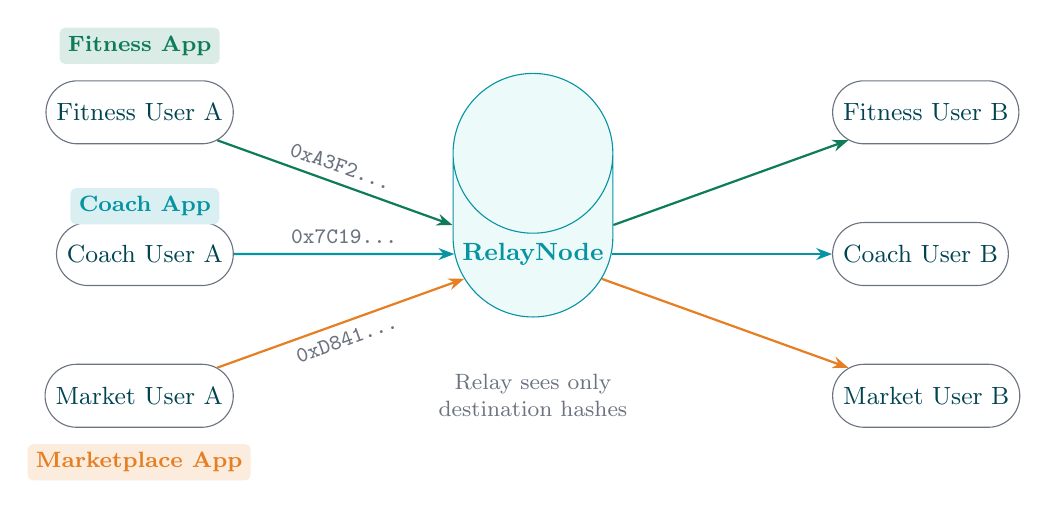
\begin{tikzpicture}[
  node distance=10mm,
  device/.style={
    rounded rectangle, draw=mwgray, fill=white,
    minimum width=22mm, minimum height=8mm,
    font=\small, text=mwblue
  },
  relay/.style={
    cylinder, shape border rotate=90,
    draw=mwaccent, fill=nodebg,
    minimum width=18mm, minimum height=14mm,
    font=\small\bfseries, text=mwaccent
  },
  blob/.style={
    font=\footnotesize\ttfamily, text=mwgray
  },
  apptag/.style={
    rounded corners=2pt, font=\footnotesize\bfseries,
    inner sep=3pt
  }
]

% Relay in the centre
\node[relay] (relay) {Relay\\Node};

% App namespaces — left side
\node[device, left=28mm of relay, yshift=18mm] (fitA) {Fitness User A};
\node[device, left=28mm of relay, yshift=-18mm] (mktA) {Market User A};
\node[device, left=28mm of relay, yshift=0mm] (coachA) {Coach User A};

% App namespaces — right side
\node[device, right=28mm of relay, yshift=18mm] (fitB) {Fitness User B};
\node[device, right=28mm of relay, yshift=-18mm] (mktB) {Market User B};
\node[device, right=28mm of relay, yshift=0mm] (coachB) {Coach User B};

% Fitness connections
\draw[-{Stealth[length=2mm]}, color=mwgreen, thick]
  (fitA) -- node[blob, above, sloped]{\texttt{0xA3F2…}} (relay);
\draw[-{Stealth[length=2mm]}, color=mwgreen, thick]
  (relay) -- (fitB);

% Coach connections
\draw[-{Stealth[length=2mm]}, color=mwaccent, thick]
  (coachA) -- node[blob, above, sloped]{\texttt{0x7C19…}} (relay);
\draw[-{Stealth[length=2mm]}, color=mwaccent, thick]
  (relay) -- (coachB);

% Marketplace connections
\draw[-{Stealth[length=2mm]}, color=mworange, thick]
  (mktA) -- node[blob, below, sloped]{\texttt{0xD841…}} (relay);
\draw[-{Stealth[length=2mm]}, color=mworange, thick]
  (relay) -- (mktB);

% App labels
\node[apptag, fill=mwgreen!15, text=mwgreen, above=2mm of fitA] {Fitness App};
\node[apptag, fill=mwaccent!15, text=mwaccent] at (coachA.north) [yshift=2mm] {Coach App};
\node[apptag, fill=mworange!15, text=mworange, below=2mm of mktA] {Marketplace App};

% "Relay sees only hashes" annotation
\node[font=\footnotesize, text=mwgray, align=center, below=6mm of relay]
  {Relay sees only\\destination hashes};

\end{tikzpicture}
\caption{Three applications share the same relay node. The relay forwards encrypted blobs identified only by rotating destination hashes — it cannot determine which application a packet belongs to, who sent it, or what it contains. The applications are cryptographically isolated from each other at the session layer.}
\label{fig:namespace}
\end{figure}

% ─────────────────────────────────────────────────────────────────────────────
\section{How the Mesh is Structured}

The network has two complementary layers.

\subsection{The Node Layer}

When a developer integrates the MeshWhisper SDK into their application, they also deploy a MeshWhisper Node — a single lightweight binary that bundles four functions into one process on one port: packet relay and store-and-forward, push notification forwarding, encrypted media storage, and a prekey directory for first contact between strangers. One Docker container. One port. Everything included.

The node handles what phones cannot: it is always on, always connectable, and holds messages for offline recipients. When a user is not running the app, the node fires a silent, content-free wake signal via APNs or FCM — the same mechanism Signal and WhatsApp use — and the device wakes, connects, and pulls its waiting messages. The node never holds a decryption key. The wake signal contains no message content. The node is, architecturally, a post box, not a postman.

Developers who prefer not to self-host can use a public-good relay --- currently the first such node, live at \texttt{relay.meshwhisper.org} --- or any other operator's relay they trust. Self-hosting is always free; the node binary is open source. Sustainability of public-good infrastructure is discussed later, in the section on operator economics.

\subsection{The Device Layer}

Every device running any SDK-embedded application is simultaneously a potential relay for every other such device. When two devices are nearby, they relay for each other directly using platform-native P2P (Apple Multipeer Connectivity on iOS, Google Nearby Connections on Android). Over the internet, devices that can accept inbound connections — laptops on broadband, desktops, home relay hardware — act as connectable peers. Phones on cellular maintain outbound connections to their deployed node.

Figure~\ref{fig:layers} shows the relationship between the two layers. The node layer forms the backbone — reliable, always-connectable bridging infrastructure. The device layer forms the mesh — organic, distributed relay capacity that grows with adoption.

\subsection{Namespace Isolation}

Applications sharing relay infrastructure are isolated from each other cryptographically, not by access control. Each application is identified by a namespace derived from the developer's public key and the application bundle identifier. Destination hashes — the routing identifiers on every packet — are computed as \texttt{BLAKE3(namespace\_id \textbar\textbar\ peer\_key \textbar\textbar\ epoch\_hour)}. A packet's destination hash is only reproducible by a party who knows the namespace identifier, which is scoped to the specific developer and application. A relay node routing packets for three different apps cannot tell them apart, cannot inject packets into any namespace without knowing the identifier, and cannot correlate traffic across namespaces even under active observation. The isolation is a structural consequence of the routing design, not a configuration option or an access policy that can be misconfigured.

\vspace{10pt}

% ── Figure 2: Two-layer architecture ──────────────────────────────────────────
\begin{figure}[h]
\centering
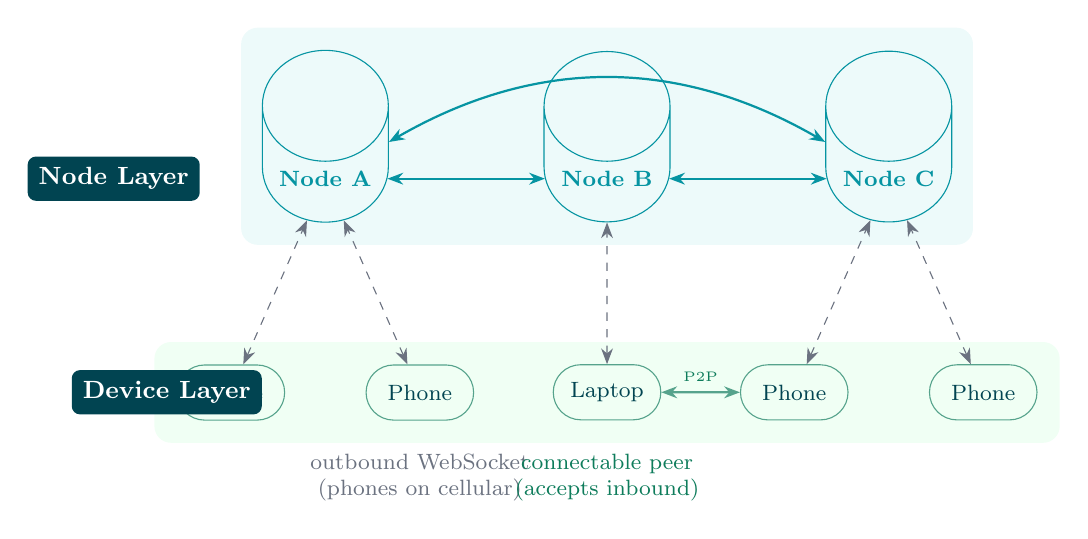
\begin{tikzpicture}[
  node distance=8mm,
  mwnode/.style={
    cylinder, shape border rotate=90,
    draw=mwaccent, fill=nodebg,
    minimum width=16mm, minimum height=12mm,
    font=\footnotesize\bfseries, text=mwaccent
  },
  phone/.style={
    rounded rectangle, draw=mwgreen!70, fill=devicebg,
    minimum width=16mm, minimum height=7mm,
    font=\footnotesize, text=mwblue
  },
  laptop/.style={
    rounded rectangle, draw=mwgreen!70, fill=devicebg,
    minimum width=16mm, minimum height=7mm,
    font=\footnotesize, text=mwblue
  },
  layerlabel/.style={
    font=\small\bfseries, text=white,
    fill=mwblue, rounded corners=3pt,
    inner sep=4pt
  }
]

% ---- Node layer ----
\node[mwnode] (n1) {Node A};
\node[mwnode, right=20mm of n1] (n2) {Node B};
\node[mwnode, right=20mm of n2] (n3) {Node C};

% Node interconnections
\draw[thick, mwaccent, {Stealth[length=2mm]}-{Stealth[length=2mm]}] (n1) -- (n2);
\draw[thick, mwaccent, {Stealth[length=2mm]}-{Stealth[length=2mm]}] (n2) -- (n3);
\draw[thick, mwaccent, {Stealth[length=2mm]}-{Stealth[length=2mm]}, bend left=30] (n1) to (n3);

% Layer label — nodes
\node[layerlabel, left=8mm of n1] {Node Layer};

% Bounding box for node layer
\begin{scope}[on background layer]
  \node[fill=nodebg, rounded corners=6pt, fit=(n1)(n2)(n3), inner sep=8pt] {};
\end{scope}

% ---- Device layer ----
\node[phone, below=18mm of n1, xshift=-12mm] (p1) {Phone};
\node[phone, below=18mm of n1, xshift=12mm] (p2) {Phone};
\node[laptop, below=18mm of n2] (l1) {Laptop};
\node[phone, below=18mm of n3, xshift=-12mm] (p3) {Phone};
\node[phone, below=18mm of n3, xshift=12mm] (p4) {Phone};

% Device layer label
\node[layerlabel, left=8mm of n1 |- l1] {Device Layer};

% Bounding box for device layer
\begin{scope}[on background layer]
  \node[fill=devicebg, rounded corners=6pt,
    fit=(p1)(p2)(l1)(p3)(p4), inner sep=8pt] {};
\end{scope}

% Devices → nodes (upward connections)
\draw[mwgray, dashed, {Stealth[length=2mm]}-{Stealth[length=2mm]}] (p1) -- (n1);
\draw[mwgray, dashed, {Stealth[length=2mm]}-{Stealth[length=2mm]}] (p2) -- (n1);
\draw[mwgray, dashed, {Stealth[length=2mm]}-{Stealth[length=2mm]}] (l1) -- (n2);
\draw[mwgray, dashed, {Stealth[length=2mm]}-{Stealth[length=2mm]}] (p3) -- (n3);
\draw[mwgray, dashed, {Stealth[length=2mm]}-{Stealth[length=2mm]}] (p4) -- (n3);

% Device-to-device (local P2P)
\draw[mwgreen!70, thick, {Stealth[length=2mm]}-{Stealth[length=2mm]}]
  (l1) -- node[font=\tiny, text=mwgreen, above, sloped]{P2P} (p3);

% Annotations
\node[font=\footnotesize, text=mwgray, align=center, below=3mm of p2]
  {outbound WebSocket\\(phones on cellular)};
\node[font=\footnotesize, text=mwgreen, align=center, below=3mm of l1]
  {connectable peer\\(accepts inbound)};

\end{tikzpicture}
\caption{The two-layer architecture. The node layer (blue) forms the backbone — nodes interconnect directly and bridge devices that cannot accept inbound connections. The device layer (green) forms the mesh — devices relay for each other over platform P2P, local network, and internet. A laptop on broadband is a connectable peer and can relay directly; a phone on cellular maintains an outbound connection to its node.}
\label{fig:layers}
\end{figure}

% ─────────────────────────────────────────────────────────────────────────────
\section{Network Effects, Honestly}

The central challenge of any mesh protocol is the bootstrap problem. A mesh that does not exist is not useful. A network effect that requires a large network to deliver value is a circular dependency.

MeshWhisper separates the problem into two layers with different timelines.

The node layer has value from the first integration. A developer who deploys a MeshWhisper Node gets working E2EE relay infrastructure for their users immediately, before any other application has integrated the SDK. That is a real outcome. But it is worth being direct: a single developer with a single node has something structurally similar to what a self-hosted Matrix homeserver or a managed Sendbird deployment already provides — reliable delivery, push notifications, and end-to-end encryption for one application's users. The node layer sets a floor, not a ceiling.

The distinctive value is in the mesh layer, and the mesh layer requires adoption that does not exist on day one. Multi-node privacy routing, ambient relay capacity, and the privacy-improves-with-scale property are all functions of how many nodes and devices are participating. That is the honest statement of the bootstrap dependency.

The path through it is not a theory. GestureLoop deploys MeshWhisper in its own applications. Those deployments create real running infrastructure — nodes, real users, real message routing. A developer evaluating the SDK is evaluating something that exists and functions, not a proposal. Each additional developer integration adds a node and an active user base, shifting the aggregate relay topology further from "one operator's infrastructure" toward "shared mesh." The transition is incremental and each step has independent value, but the full value proposition requires the mesh that adoption builds.

This is the BitTorrent dynamic honestly applied. BitTorrent had no peers for the first torrent. MeshWhisper has no mesh for the first integration. What the architecture ensures is that each stage of adoption — from single-node to multi-node to dense mesh — delivers real, usable value to the developer who integrates at that stage. The ceiling scales with adoption; the floor is set on day one.

% ─────────────────────────────────────────────────────────────────────────────
\section{Privacy That Strengthens With Scale}

This is the property that most distinguishes MeshWhisper from every centralised alternative: \textbf{privacy improves as the network grows.}

To understand why, consider what a node operator can observe. A node sees the devices directly connected to it — their source IP addresses, push tokens, and the timing of their traffic. It also sees destination hashes (rotating hourly identifiers that do not persist across time periods) and the volume of traffic it forwards between other nodes. It does not see message content, sender identity, or recipient identity. It does not know which application a packet belongs to.

Traffic timing is partially obscured by a second mechanism. Every active device generates a continuous stream of random encrypted packets — chaff — regardless of whether the user is sending real messages. The rate is proportional to the device's relay willingness setting but is constant rather than activity-correlated. A node operator observing a device cannot distinguish real messages from background noise, and cannot infer from traffic volume alone whether a conversation is actively in progress. The side effect of this privacy measure is that total traffic volume from a node's connected devices is proportional to the number of active devices rather than to message activity, which is relevant to capacity planning and billing.

\subsection{Low density: the weakest case}

At low mesh density, a sender and recipient may share the same node. Alice's device connects to Node X. Bob's device also connects to Node X. A message travels Alice → Node X → Bob. Node X sees both endpoints. It can observe that traffic flowed between them. This is the weakest privacy case — equivalent to using a centralised messaging service, minus the ability to read content.

\subsection{High density: the strong case}

As mesh density increases — more applications integrating, more nodes deployed, more devices participating — paths between senders and recipients lengthen and diversify. Figure~\ref{fig:privacy} illustrates the contrast.

Alice and Bob now have different nodes. Alice's node (Node A) sees Alice's IP, her push token, and that she sent a message. Bob's node (Node C) sees Bob's IP, his push token, and that he received a message. An intermediate node (Node B) sees only two adjacent node connections and some traffic volume. No single party holds enough information to reconstruct the conversation.

At higher density still, paths route through several intermediate nodes, none of which see either endpoint. The metadata is distributed across multiple independent parties, each holding a fragment too small to be useful to an adversary.

\vspace{10pt}

% ── Figure 3: Privacy at low vs high density ──────────────────────────────────
\begin{figure}[h]
\centering

% ---- Low density ----
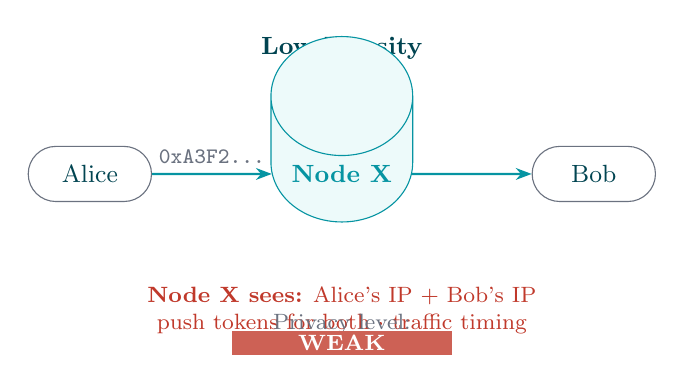
\begin{tikzpicture}[
  device/.style={
    rounded rectangle, draw=mwgray, fill=white,
    minimum width=18mm, minimum height=7mm,
    font=\small, text=mwblue
  },
  mwnode/.style={
    cylinder, shape border rotate=90,
    draw=mwaccent, fill=nodebg,
    minimum width=18mm, minimum height=13mm,
    font=\small\bfseries, text=mwaccent
  },
  seeslabel/.style={font=\footnotesize, text=mwred},
  blindlabel/.style={font=\footnotesize, text=mwgreen}
]

% LOW DENSITY
\node[font=\small\bfseries, text=mwblue] at (0, 1.6) {Low Density};

\node[device] (aliceL) at (-3.2, 0) {Alice};
\node[mwnode] (nodeL) at (0, 0) {Node X};
\node[device] (bobL) at (3.2, 0) {Bob};

\draw[thick, mwaccent, -{Stealth[length=2mm]}]
  (aliceL) -- node[above, font=\footnotesize\ttfamily, text=mwgray]{\texttt{0xA3F2…}} (nodeL);
\draw[thick, mwaccent, -{Stealth[length=2mm]}] (nodeL) -- (bobL);

% What Node X sees
\node[seeslabel, align=center, below=7mm of nodeL]
  {\textcolor{mwred}{\textbf{Node X sees:}} Alice's IP + Bob's IP\\push tokens for both · traffic timing};

% LOW DENSITY privacy bar
\node[font=\footnotesize, text=mwgray] at (0, -1.9) {Privacy level:};
\fill[mwred!80] (-1.4, -2.3) rectangle (1.4, -2.0);
\node[font=\footnotesize\bfseries, text=white] at (0, -2.15) {WEAK};

\end{tikzpicture}

\vspace{8mm}

% HIGH DENSITY
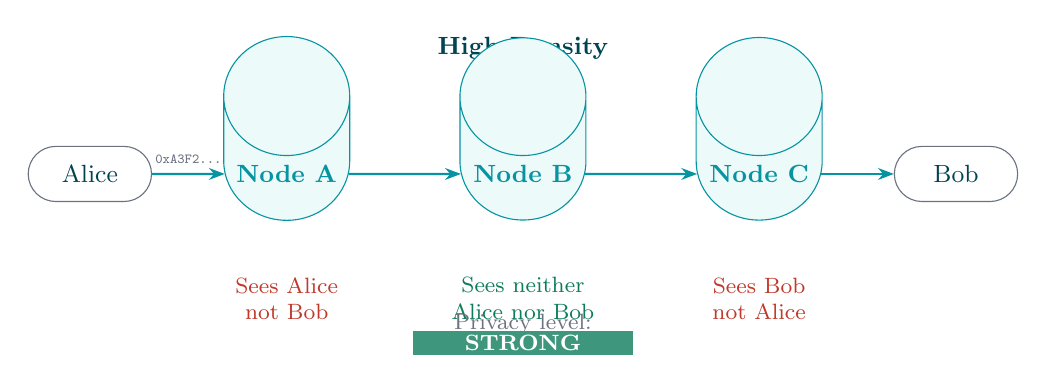
\begin{tikzpicture}[
  device/.style={
    rounded rectangle, draw=mwgray, fill=white,
    minimum width=18mm, minimum height=7mm,
    font=\small, text=mwblue
  },
  mwnode/.style={
    cylinder, shape border rotate=90,
    draw=mwaccent, fill=nodebg,
    minimum width=16mm, minimum height=12mm,
    font=\small\bfseries, text=mwaccent
  }
]

\node[font=\small\bfseries, text=mwblue] at (0, 1.6) {High Density};

\node[device] (aliceH) at (-5.5, 0) {Alice};
\node[mwnode] (nodeA) at (-3.0, 0) {Node A};
\node[mwnode] (nodeB) at (0, 0) {Node B};
\node[mwnode] (nodeC) at (3.0, 0) {Node C};
\node[device] (bobH) at (5.5, 0) {Bob};

\draw[thick, mwaccent, -{Stealth[length=2mm]}]
  (aliceH) -- node[above, font=\tiny\ttfamily, text=mwgray]{\texttt{0xA3F2…}} (nodeA);
\draw[thick, mwaccent, -{Stealth[length=2mm]}] (nodeA) -- (nodeB);
\draw[thick, mwaccent, -{Stealth[length=2mm]}] (nodeB) -- (nodeC);
\draw[thick, mwaccent, -{Stealth[length=2mm]}] (nodeC) -- (bobH);

% What each node sees
\node[font=\footnotesize, text=mwred, align=center, below=6mm of nodeA]
  {Sees Alice\\not Bob};
\node[font=\footnotesize, text=mwgreen, align=center, below=6mm of nodeB]
  {Sees neither\\Alice nor Bob};
\node[font=\footnotesize, text=mwred, align=center, below=6mm of nodeC]
  {Sees Bob\\not Alice};

% HIGH DENSITY privacy bar
\node[font=\footnotesize, text=mwgray] at (0, -1.9) {Privacy level:};
\fill[mwgreen!80] (-1.4, -2.3) rectangle (1.4, -2.0);
\node[font=\footnotesize\bfseries, text=white] at (0, -2.15) {STRONG};

\end{tikzpicture}

\caption{Privacy as a function of mesh density. At low density (top), a message may route through a single shared node that sees both endpoints. At high density (bottom), messages route through multiple nodes: Alice's node sees only Alice, Bob's node sees only Bob, and intermediate nodes see neither. No single party can reconstruct the conversation. This improvement happens automatically as adoption grows — no additional engineering is required.}
\label{fig:privacy}
\end{figure}

\subsection{The inversion of the usual assumption}

With centralised messaging, scale makes privacy worse. A larger Signal or WhatsApp is a larger honeypot — more metadata concentrated in one place, more value in compromising it, more pressure from governments demanding records. The privacy guarantee depends on trusting a single party that becomes an increasingly attractive target as it grows.

With MeshWhisper, scale makes privacy better. More applications integrating means more nodes. More nodes means longer average paths. Longer paths means each node's view of any conversation narrows. The metadata is distributed across more parties, each holding a smaller and less useful fragment.

\begin{pullquote}
The security model strengthens organically as a side effect of adoption. Each new application that integrates the SDK is, without any intent, making every existing user's communications harder to surveil.
\end{pullquote}

This is not a privacy feature that has to be maintained against the pressures growth creates. It is a structural property of the protocol that improves automatically and requires no action from developers or users.

% ─────────────────────────────────────────────────────────────────────────────
\section{What This Enables}

The immediate consequence is economic. Messaging currently costs developers either months of engineering time or hundreds of dollars per month in perpetuity. MeshWhisper makes messaging the same kind of infrastructure decision as authentication or analytics — something you integrate in an afternoon with a library, not something you build or pay ongoing costs to operate.

\vspace{8pt}

% ── Developer integration overview ───────────────────────────────────────────
\begin{mdframed}[
  backgroundcolor=mwlight,
  linecolor=mwaccent,
  linewidth=0.8pt,
  innerleftmargin=14pt,
  innerrightmargin=14pt,
  innertopmargin=10pt,
  innerbottommargin=10pt,
  roundcorner=4pt
]
\textbf{\color{mwblue}Developer integration at a glance}

\vspace{6pt}

\begin{tabularx}{\linewidth}{@{}>{\bfseries}lX@{}}
\toprule
Step & What you do \\
\midrule
1.\ Deploy  & \texttt{docker run -p 8080:8080 meshwhisper/node} — one container, one port \\[3pt]
2.\ Install & \texttt{npm install @meshwhisper/sdk} \\[3pt]
3.\ Init    & \texttt{MeshWhisper.init(\{ namespace: 'com.myapp',}\\
            & \texttt{\phantom{MeshWhisper.init(\{ }node: 'wss://my-node.example.com' \})} \\[3pt]
4.\ Send    & \texttt{await MeshWhisper.sendMessage(recipientId, payload)} \\[3pt]
5.\ Receive & \texttt{onMessage: (msg) => display(msg)} \\
\bottomrule
\end{tabularx}

\vspace{10pt}

\begin{tabularx}{\linewidth}{@{}XX@{}}
\toprule
\textbf{\color{mwblue}Your app owns} & \textbf{\color{mwblue}MeshWhisper owns} \\
\midrule
User accounts and identity & Cryptographic key exchange (PQXDH) \\
Message content (E2EE — no one sees it) & Session encryption (Double Ratchet) \\
Your deployed Node & Packet routing and relay logic \\
Your users' data & Store-and-forward for offline recipients \\
Your application UI and product & Push notification dispatch \\
 & Post-quantum security stack \\
\bottomrule
\end{tabularx}
\end{mdframed}

\vspace{6pt}

\textbf{The long tail of apps that should have messaging but don't.} The current economics of messaging ration the feature to well-resourced teams. Well-funded consumer apps can afford Sendbird. Enterprise vendors can build custom infrastructure. Everyone else redirects users to WhatsApp or ships without the feature. MeshWhisper breaks this stratification. A solo developer building a niche community app, an NGO deploying a coordination tool, a researcher building a protocol study app — all get access to the same messaging infrastructure as a funded startup. The cost barrier disappears.

\textbf{Privacy as a default, not a premium.} Every message sent through MeshWhisper is end-to-end encrypted before it leaves the device. The protocol uses a hybrid classical and post-quantum cryptographic stack: X3DH key exchange extended with ML-KEM-768 encapsulation (PQXDH), followed by Double Ratchet session encryption. This meets what Apple calls Level~2 post-quantum security — the same class as the current shipping version of iMessage — protecting against adversaries who record encrypted traffic today and attempt to decrypt it with a future quantum computer. The next security milestone on the roadmap is Level~3: periodic ML-KEM injection into the ratchet itself, so that a session heals automatically after compromise rather than remaining exposed for its full lifetime. No relay node, including the Foundation and including self-hosted nodes, can read message content or identify participants beyond rotating hourly hashes. This is not a configuration option. There is no plaintext mode. A developer who integrates MeshWhisper has post-quantum E2EE messaging without having to understand cryptography, implement it, or make any decision about it. The default is privacy.

\textbf{Resilience where infrastructure is unreliable.} The protocol's multi-bearer transport — platform-native P2P, local network, internet — degrades gracefully as connectivity degrades. Two devices on the same subnet can message each other when the internet is down. Two devices physically nearby can communicate without any network infrastructure using platform P2P. This is not primarily a disaster-response feature, though it applies there. It is a structural property that means an app built on MeshWhisper functions in rural areas with intermittent connectivity, in buildings with poor cellular coverage, and at events where networks are congested.

\textbf{The mesh as a side effect of existence.} As adoption grows, a device running any SDK-embedded application is contributing to relay infrastructure for every other SDK-embedded application. A fitness app's users are part of the relay backbone for a marketplace app's users, and vice versa. This is the protocol's most unusual property: the infrastructure is built by participation, not by investment. The aggregate of ordinary developers adding a messaging library to their applications is an ambient messaging infrastructure that nobody had to build directly.

% ─────────────────────────────────────────────────────────────────────────────
\section{What It Is Not}

MeshWhisper is not fully serverless in the engineering sense. The MeshWhisper Node is a server. Public-good relays are servers. Developers self-hosting their own nodes are running servers. The protocol is honest about this.

What it is serverless for is the developer experience. A developer integrating the SDK does not need to build, scale, or maintain messaging infrastructure. They deploy one Docker container (or use the Foundation's) and add ten lines of code to their application. The infrastructure complexity is solved once, at the protocol level, and reused by every integration.

The distinction matters because honesty about infrastructure is what makes the trust model credible. MeshWhisper's nodes are explicitly part of the architecture, with a precisely defined threat model: they relay opaque encrypted blobs, hold rotating destination hashes, and store push tokens for offline delivery. They are ISPs carrying encrypted traffic, not parties to the conversation.

MeshWhisper is also not anonymous communication in the strong sense. It is not Tor. A node operator can observe the devices directly connected to it — their IP addresses, push tokens, and traffic timing. What they cannot observe is the full path of any given conversation, and as density increases, even the partial view narrows. Users who require strong anonymity guarantees at any density level should use a VPN alongside the SDK.

The honest framing is: at low density, MeshWhisper provides strong content privacy with moderate metadata privacy. At high density, it provides strong content privacy and strong metadata privacy. The trajectory is consistently toward stronger privacy as adoption grows, and it gets there without any action required from developers or users.

\subsection*{How it compares to open alternatives}

A developer who knows the open-protocol landscape deserves a direct comparison rather than silence on the subject.

\textbf{Matrix / Element} is federated, supports E2EE, and has real developer adoption. The differences are structural. Matrix homeservers store the full history of every encrypted room — a homeserver operator who disables or misconfigures E2EE can read all content, and the federation model means messages traverse multiple servers by design. Matrix has no device-layer mesh: devices connect to homeservers, and all traffic routes through servers. The namespace model is per-homeserver, and federation means users across homeservers are co-visible within shared rooms. MeshWhisper's relay is content-blind and namespace-blind by construction — the node cannot determine which application a packet belongs to, cannot form a view of conversation graphs, and has no persistent message storage.

\textbf{Nostr} relays see public keys, event content, and timestamps — it is designed for public broadcast and has no inherent privacy model for private messaging. The relay architecture is similar in shape (publish-subscribe rather than relayed E2EE sessions), but the threat model is fundamentally different.

\textbf{XMPP} is the oldest federated alternative. E2EE via OMEMO is available but optional and inconsistently deployed across clients. The federation model shares Matrix's characteristics. No device-layer mesh exists.

The comparison that most directly tests MeshWhisper's claims is Matrix. If the use case is a standalone federated messaging system and users will manage accounts directly, Matrix is a mature choice. MeshWhisper is designed for a different deployment pattern: a library that sits inside an existing application, uses the application's existing identity and user model, is invisible to users as infrastructure, and accumulates ambient relay capacity as a side effect of deployment. These are different tools for different problems, and a developer who has read this far should be able to tell which one fits their situation.

\subsection*{Backup that doesn't betray the protocol}

Most messengers solve cross-device continuity by exporting an encrypted backup to a third-party cloud — Google Drive, iCloud, a homeserver, the developer's own backup service. The backup itself is opaque to that third party, but its existence is not. Cloud providers learn that a given user has a WhatsApp backup, when it was made, and how large it is. For a protocol that goes to architectural lengths to prevent any single party from holding both ends of a conversation, leaking that metadata to a separate provider is a significant give-back.

MeshWhisper's archive design avoids this. Backup colocates with the relay the user has already chosen to trust. The archive is a single AES-GCM blob, keyed by the user's peer ID, stored alongside the rest of the relay's opaque content. The relay sees no account, no email, no phone number, no username — only an unidentified peer-ID hash and an encrypted payload. The backup encryption key and the write-authentication token are both HKDF-derived from the user's identity key, which is itself derived from the username and password via PBKDF2. The user does not separately manage a recovery code, a security key, or a third-party account; the password they already use to unlock the application is sufficient to recover their full conversation history on any device. Sessions are intentionally excluded from the archive so that a stolen backup cannot decrypt past or future traffic — forward secrecy is preserved even at rest.

\vspace{4pt}
\begin{center}
\small
\renewcommand{\arraystretch}{1.25}
\begin{tabular}{>{\bfseries}l p{42mm} p{52mm} p{38mm}}
\toprule
\rowcolor{mwlight}\color{mwblue}Approach & \color{mwblue}\bfseries Where backup lives & \color{mwblue}\bfseries Who sees metadata & \color{mwblue}\bfseries Recovery requires \\
\midrule
MeshWhisper & The same relay you already use for messaging & Relay sees an opaque blob keyed by an unidentified peer-ID hash. No account, email, or phone number. & Username + password \\
WhatsApp    & Google Drive / iCloud & Google or Apple sees that you have a WhatsApp backup, when, and how big & Phone number + (optional) E2EE key \\
Signal      & Local device or paired-device transfer only & Nothing — but no off-device backup historically & Local backup file with passphrase \\
iMessage    & iCloud & Apple holds keys (default) or user-held with Advanced Data Protection & Apple ID \\
Matrix      & Homeserver-stored encrypted key backup & Your homeserver knows the backup exists, who owns it, and its timing & Security key or passphrase \\
\bottomrule
\end{tabular}
\end{center}
\vspace{4pt}

The result is a backup model with the same trust shape as the rest of the protocol. If the user self-hosts the relay, they self-host the backup. If they use a Foundation relay, the Foundation sees the same opaque blob it already routes for live traffic — nothing new becomes visible. This is qualitatively different from the standard pattern of ``encrypted messaging app, plus a separate cloud account that knows you use it.''

\subsection*{Operator economics, in three layers}

Infrastructure economics and application economics are different problems and shouldn't be conflated. App developers monetise through their products. The protocol intentionally avoids any per-message-volume or per-user-count tax that an app would have to absorb out of its product margin. The same dynamic that makes Sendbird and PubNub painful --- paying a layered cost to operate a feature your app needs --- is exactly what MeshWhisper exists to escape.

The right question is how the \emph{infrastructure} sustains itself, on its own terms, by parties with direct interest in operating infrastructure. Three layers, with their own economics:

\textbf{The protocol layer.} MIT-licensed, free, anyone can implement, anyone can extend. No commercial relationship with anyone is required to use it. This stays the case forever.

\textbf{The infrastructure layer.} Anyone runs a relay node. The first such node is live at \texttt{relay.meshwhisper.org}, alongside Prudence (the reference PWA at \texttt{prudence.meshwhisper.org}). A public-good Foundation may eventually formalise as a non-commercial entity that operates backbone capacity funded by donations, grants, or aligned commercial sponsors --- the same shape Mozilla Foundation, the Tor Project, or ICANN occupy in their domains. We are explicitly not proposing a freemium-on-Foundation model with per-MAU pricing, because that would create economic pressure for everyone to centralise on whoever runs the freemium tier --- directly opposing the privacy-through-density property the protocol depends on.

\textbf{The commercial-services layer.} Anyone can offer managed hosting, enterprise support, or custom deployment as a commercial service. This is a competitive market, not a protocol tax. Managed hosting competes on quality and price the way managed Postgres or managed Redis competes; it doesn't have privileged status, and it doesn't extract from app developers. A developer who wants to outsource ops pays a hosting provider; a developer who wants control runs the binary themselves; both paths remain first-class.

The trap to name explicitly: a per-MAU tier on whatever entity ends up hosting public-good infrastructure would push every small developer toward that infrastructure, fragment the operator base, and undermine the whitepaper's strongest privacy claim. We're avoiding it by design.

\subsection*{Why operators open their nodes}

The protocol asks every operator to forward encrypted packets regardless of which application they belong to. There are three reasons to participate, in roughly increasing strength:

\textbf{Philosophy.} You believe a content-blind, multi-operator messaging substrate is worth contributing to. Same energy that runs Tor middle nodes and seeds open-source torrents.

\textbf{Reciprocity for your own privacy.} The privacy property that ``no single operator sees both ends of a conversation'' only activates when \emph{your} users' messages can route through other operators. If you don't forward theirs, you don't get to expect them to forward yours. Selfish operators get a worse privacy posture for their own users.

\textbf{Marginal cost.} The bandwidth involved in forwarding others' opaque blobs is small relative to a typical VPS budget. A €4 VPS typically includes ample bandwidth that a small app uses a fraction of. Closing your node saves you almost nothing and removes you from the mesh property entirely.

Promiscuous relay does not mean uncapped relay. The current reference implementation forwards openly without any reciprocity enforcement --- the closest analog is Tor's middle-node model, where operators contribute capacity without expecting tit-for-tat accounting. Adaptive throttling --- protecting a small operator from being overwhelmed by a much larger app's traffic --- is a future direction, not a v1 feature. The reasoning: at low density that protection matters in theory but the load isn't actually present; at higher density the load spreads naturally across more operators and any single node carries a smaller share. The architecture relies on operators collectively maintaining the relay-promiscuously norm; the protocol can encourage but not enforce.

% ─────────────────────────────────────────────────────────────────────────────
\section{Beyond Human Messaging}

The preceding sections frame MeshWhisper as developer infrastructure for human communication. That framing is accurate as a starting point but understates the protocol's generality.

The core primitive — authenticated, asynchronous, end-to-end encrypted message delivery between parties that have exchanged keys, without a trusted central broker, with store-and-forward for intermittently connected recipients — is not specific to human users. It applies wherever those properties are needed.

\textbf{Smart home and IoT devices.} Most smart home products communicate through the manufacturer's cloud. A light switch command travels from your phone to a server in another country and back — the manufacturer observes your usage patterns, the service can be discontinued, and a server breach potentially exposes every customer's home activity. A device with a key pair participates in PQXDH key exchange the same way a human user does. Commands from a phone to a thermostat are end-to-end encrypted before they leave the phone; the relay sees only an opaque blob. The local-network transport means commands route directly between devices on the same subnet without any internet round-trip, and the system continues to function when the internet is unavailable. MeshWhisper makes it possible to build smart home products where the manufacturer's server is relay infrastructure — not a trusted intermediary with a full record of your home's activity.

The post-quantum security properties are particularly relevant for embedded devices. A thermostat deployed today may run for ten years without a meaningful software update. Unlike a human conversation, which has a natural end, a machine session can run indefinitely — a compromised ratchet state on a long-lived device exposes all future traffic for the device's entire remaining lifetime. The planned Level~3 ratchet — periodic ML-KEM injection that heals a session automatically after compromise — bounds that exposure window regardless of how long the device runs. This is a stronger argument for ratchet-level post-quantum security in IoT than it is in human messaging.

\textbf{AI agent coordination.} Autonomous agents that need to coordinate — passing tasks, returning results, requesting tools from other agents — need a communication layer that handles authentication and asynchronous delivery. The PQXDH identity model means an agent can cryptographically verify it is communicating with the intended counterpart, not an impersonator, which is a problem most current agentic frameworks leave unsolved. Namespace isolation means multiple agent systems can share relay infrastructure without cross-contamination. Asynchronous delivery handles agents that run on different schedules or are intermittently available.

\textbf{Supply chain and logistics.} Events that need to travel between parties who do not share infrastructure and should not trust each other's servers — custody transfers, cold-chain temperature records, delivery confirmations — fit the protocol model naturally. Each party operates their own node. Events are cryptographically authenticated by the originating device, delivered asynchronously to the recipient, and the relay cannot read or correlate the data.

\textbf{Industrial and field systems.} Sensors, actuators, and controllers in environments with intermittent connectivity — remote infrastructure, maritime systems, field equipment — require reliable store-and-forward delivery, authenticated commands that a relay cannot forge or modify, and local-network routing when internet connectivity is unavailable. These are structural properties of the protocol, not features that need to be added.

In each case, the protocol's value derives from the same source: the relay does not need to read a message to route it, and a relay that cannot read a message cannot be compelled to expose it, cannot be breached to reveal it, and cannot be discontinued in a way that prevents the parties from communicating directly.

% ─────────────────────────────────────────────────────────────────────────────
\section{The Protocol's Place}

The history of the internet is a history of protocols becoming ambient infrastructure. SMTP is not a product — it is infrastructure that email products are built on. DNS is not a product — it is infrastructure that every internet application uses. HTTP is not a product — it is infrastructure that the web is built on. No individual company operates these protocols. No single party controls them. They exist as shared utilities, maintained by open specifications, implemented by competing and cooperating parties, and used by applications that neither know nor care about the underlying mechanics.

Messaging has not had its SMTP moment. The dominant messaging infrastructure is owned by a small number of large platforms, each operating closed proprietary systems, each holding the plaintext of every message their users send. Adding messaging to an application means becoming dependent on one of these platforms or building from scratch.

MeshWhisper is an attempt to give messaging its SMTP moment: an open protocol, implemented as a developer library, operated as shared infrastructure, with no single party controlling the network or able to read its traffic. One that gets better — faster, more reliable, and more private — as more developers use it. One that does not require any individual developer to understand its internals to benefit from it.

The SMTP analogy is instructive but cuts both ways. SMTP succeeded partly because institutions — universities, then ISPs — had structural incentives to run mail servers before there was a meaningful network to participate in. MeshWhisper's adoption chain is similar in shape and worth naming directly.

\textbf{Stage one} is bootstrap: GestureLoop deploys MeshWhisper in its own applications, creating real running infrastructure with real users. The first relay node is live at \texttt{relay.meshwhisper.org} alongside Prudence --- a reference PWA messaging application built entirely on the SDK, available at \texttt{prudence.meshwhisper.org}. MeshWhisper is being integrated into existing GestureLoop applications. A developer evaluating the SDK at this stage finds a working relay network with active users, not a proposal.

\textbf{Stage two} is early developer adoption: other developers integrate the SDK, deploy nodes for their own applications, and expand the relay topology. Multi-node privacy routing becomes real — messages begin to route across independent operators rather than through a single party. The bootstrap operator's share of total relay capacity shrinks as developer-deployed infrastructure grows.

\textbf{Stage three} is mesh density: as the SDK-embedded user base across all applications grows, device-layer relay capacity becomes meaningful. Delivery latency drops on short-range paths. The privacy properties of multi-hop routing become the typical case rather than the exceptional one.

Each stage has independent value for the developer who integrates at that stage. None of them require any action from users. The ceiling scales with adoption; the floor is set by the node layer on day one.

Whether the full arc is reached depends on execution. The technical foundation is in place. The first stage is already live.

% ─────────────────────────────────────────────────────────────────────────────
\section{History}

MeshWhisper began as a late-night text-message conversation between Anton Mannering and Kevin Collins. Anton proposed an end-to-end-encrypted peer-to-peer messaging protocol and sent over a PRD. Kevin had been drafting one independently from the same conversation; he combined them, and within thirty minutes a working prototype existed --- a long way from usable, but a real running starting point. Anton has architected the protocol and led its evolution since, adapting the idealised design to the realities of mobile devices, intermittent connectivity, and modern threat models.

\subsection*{From prototype to protocol}

The first commit landed at 00:18 on 10 April 2026 --- a 27-file, 11{,}693-line drop that implemented the protocol's outline end-to-end: X3DH, Double Ratchet, packet framing, transports, routing, relay logic, namespace isolation. It was an impressive sketch and an unusable product. It had no persistence, no post-quantum layer, no standalone relay server, no browser support, no push notifications, and a single test file. Most of the work since has been turning that sketch into something that survives real devices: persisting state across restarts, splitting the relay into a deployable server with SQLite-backed durability, adding PQXDH and ML-KEM-768, building a push pipeline that preserves end-to-end encryption, writing tests that found bugs that code review missed (an OPK derivation mismatch, \texttt{Math.random} used where a CSPRNG was required), designing a multi-device archive, and deferring the speculative modules that hadn't earned their place. The current codebase is many orders of magnitude removed from that first commit; the original repository is preserved in git history for anyone who wants to see the distance.

\subsection*{Implementation status, honestly}

Some layers are production: end-to-end encryption (PQXDH + Double Ratchet), persistence, push notifications, group messaging, encrypted media, the multi-device archive, safety numbers. Other layers are \emph{scaffolded} --- they sketch how the protocol intends to handle problems that emerge at scale, but they aren't load-bearing in current deployments and we don't claim otherwise. Sybil resistance for relay reputation, social-graph-aware routing, and audit-log compliance hooks all fall into this category. They are real interfaces with real designs, awaiting the conditions under which they need to be activated. As the protocol moves into the multi-operator regime described above, these layers will be hardened in step.

% ─────────────────────────────────────────────────────────────────────────────
\vspace{16pt}
\hrule
\vspace{10pt}
{\small
MeshWhisper is open source. The protocol specification, SDK, and node binary are published under the MIT licence.\\
SDK: \texttt{npm install @meshwhisper/sdk}\quad·\quad Node: available as a Docker image\quad·\quad Self-hosting is free, always.\\
Live: \texttt{relay.meshwhisper.org}\quad·\quad Reference app: Prudence (\texttt{prudence.meshwhisper.org})

\vspace{6pt}
\texttt{anton@gestureloop.com}
}

\end{document}
